
{Introduction to R}
Source: R project website (http://www.r-project.org)

* R is a language and environment for statistical computing and graphics. It is a GNU project
which is similar to the S language and environment which was developed at Bell Laboratories
(formerly AT\&T, now Lucent Technologies) by John Chambers and colleagues. 
* R can be considered
as a different implementation of S. There are some important differences, but much
code written for S runs unaltered under R.




%===

{What is R?}

* R provides a wide variety of statistical (linear and nonlinear modelling, classical statistical tests,
time-series analysis, classification, clustering, ...) and graphical techniques, and is highly extensible.
* The S language is often the vehicle of choice for research in statistical methodology,
and ``R} provides an Open Source route to participation in that activity.
* One of ``R}’s strengths is the ease with which well-designed publication-quality plots can be
produced, including mathematical symbols and formulae where needed. 




%===

{What is R?}

* Great care has been
taken over the defaults for the minor design choices in graphics, but the user retains full control.
* ``R} is available as Free Software under the terms of the Free Software Foundation’s GNU General
Public License in source code form. It compiles and runs on a wide variety of UNIX platforms
and similar systems (including FreeBSD and Linux), Windows and MacOS.


%===


{What is R?}
``R} is a programming environment that

* uses a well-developed but simple programming language
* allows for rapid development of new tools according to user demand
* these tools are distributed as packages, which any user can download to customize the R
environment.


%===

% % SLIDE 1 - COVER SLIDE
\begin{figure}
\centering
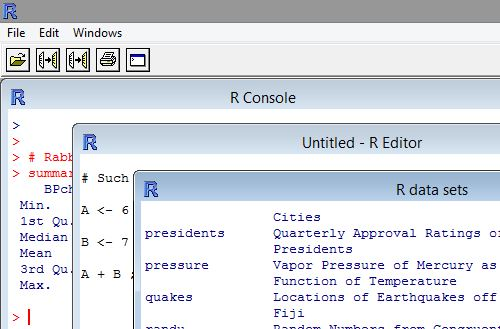
\includegraphics[width=1.2\linewidth]{images/Rmultiplewindows}
\end{figure}

   

%===

{Comprehensive R Archive Network}

* Base ``R} and most ``R} packages are available for download from the \textbf{Comprehensive R Archive Network}
(CRAN) cran.r-project.org. 
* Base ``R} comes with a number of basic data management,
analysis, and graphical tools 
* ``R}s power and flexibility, however, lie in its array of packages
(currently more than 6,000!)



%========== %
 
\begin{figure}
\centering
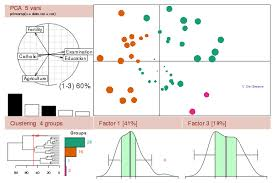
\includegraphics[width=1.2\linewidth]{CRAN}
\end{figure}

% %

{Introduction to R}
\textbf{Secton 1 - A few basics} 

\item[1.1] Installing ``R}      
\item[1.2] Command Line Interface     
\item[1.3] The Assignment operator     
\item[1.4] Commenting      
\item[1.5] Defining Variables     
\item[1.6] Help Functions      
\item[1.7] The ``help.start()`` command     
\item[1.8] Basic Maths Operations     
\item[1.9] Basic ``R} Editor      


%===

{1.1 Installing R}

* ``R} is very easily installed by downloading it from the CRAN website. Installation usually takes
about 2 minutes. 
* When installation of R is complete, the distinctive ``R} icon will appear on your
desktop. To start ``R}, simply click this Icon. 
* It is common to re-install ``R} once a year or so. The
current version of ``R}, version 3.1.2 was released quite recently.





%===

% % SLIDE 1 - COVER SLIDE
\begin{figure}
\centering
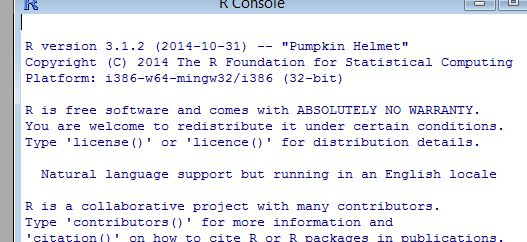
\includegraphics[width=1.2\linewidth]{images/Rversion}        
\end{figure}
  
%===


{1.2 Command Line Interface}

* When you start ``R}, the command line interface window will appear on screen. This is one
of many windows in the ``R} environment, others including graphical output windows, or script
editors. 
* ``R} code can be entered into the command line directly. 
* Alternatively code can be saved
to a script, which can be run inside a session using the ``source()`` function.


%===

{1.3 The Assignment operator}

* The assignment operator is used to assign names to particular values. 
* Historically the assignment
operator was ) a ````$<-$}”. 
* The assignment operator can also be the equals sign "=". (This is valid as of ``R}
version 1.4.0.)

* Both will be used, although, you should learn one and stick with it. Many long term ``R}
users prefer the arrow approach. 



%===

{1.3 The Assignment operator}

* You can also use $->$ as an assignment operator, reversing the
usual assignment positions. (This is actually really useful).
* Commands are separated either by
a semi colon or by a newline.

\begin{figure}
\centering
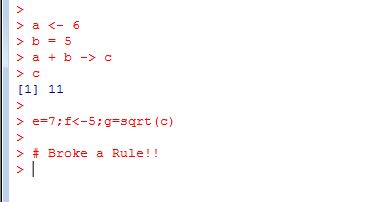
\includegraphics[width=1.2\linewidth]{images/assignment}
%\caption{}
%\label{fig:assignment}
\end{figure}



%===

{1.3 The Assignment operator}
\textbf{The Up and Down Keys}

* Before we continue, try using the up and down keys, and see what happens. 
* Previously
typed commands are re-presented, and can be re-executed.



%===

{1.3 The Assignment operator }
\textbf{objects}

* R stores both data and output from data analysis (as well as everything else) in \textbf{objects}.
* The variables we have created so far are objects. 
* A list of all objects in the current session can
be obtained with ``ls()``.


\textbf{1.3.1 Reserved Words - Bad names for Objects}

* Some names are used by the system, e.g.``T, F,q,c} etc . 
* Avoid using these. (This is the rule I broke earlier on)
* Also avoid using command names like \textbf{mean} and \textbf{sum}



  
%===

{1.4 Commenting}
For the sake of readability, it is good practice to comment code. The \# character at the
beginning of a line signifies a comment, which is not executed. Lines of hashtags can be used
to identify the beginning and end of code segments
\begin{figure}
\centering
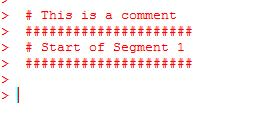
\includegraphics[width=1.2\linewidth]{images/commenting}
%\caption{}
%\label{fig:commenting}
\end{figure}


%===

{1.5 Defining and Naming Variables}

* A convention is to use define a variable name with a capital letter (R is case sensitive). 
* This
reduces the chance of overwriting in-build ``R} functions, which are usually written in lowercase
letters. 
* Commonly used variable names such as x, y and z (in lower case letters) are not “reserved”.

\textbf{Camel Case}
\begin{framed}
``camelCase}

``variableName}

``AlsoCamelCase}
\end{framed}


%===


{1.6 Help Functions}

*  Help files for R functions are accessed by preceding the name of the function with ?\\  (e.g. ``?sort}
). 

* Alternatively you can use the command ``help()`` (e.g. ``help(sqrt)} )



%===


{1.6 Help Functions}

* A HTML document appears on screen with information on the function typed in. 
* As well
as the list of arguments that the particular function accepts, and how to specify them, there is
example code at the bottom of the file. 
* These code segments are often invaluable in learning
how to master the function.





%===

% % SLIDE 1 - COVER SLIDE
\begin{figure}
\centering
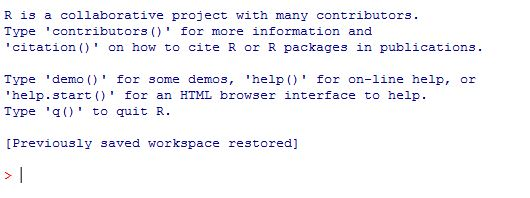
\includegraphics[width=1.2\linewidth]{images/Rhelpcommands}
%%\caption{}
%%\label{fig:Rhelpcommands}
\end{figure}
   


 
%===



{1.7 The ``help.start()`` command}
As mentioned by the text on the main console, the ``help.start()`` command can be usd to
access detailed help documentation that comes as part of the installation.


\begin{figure}
\centering
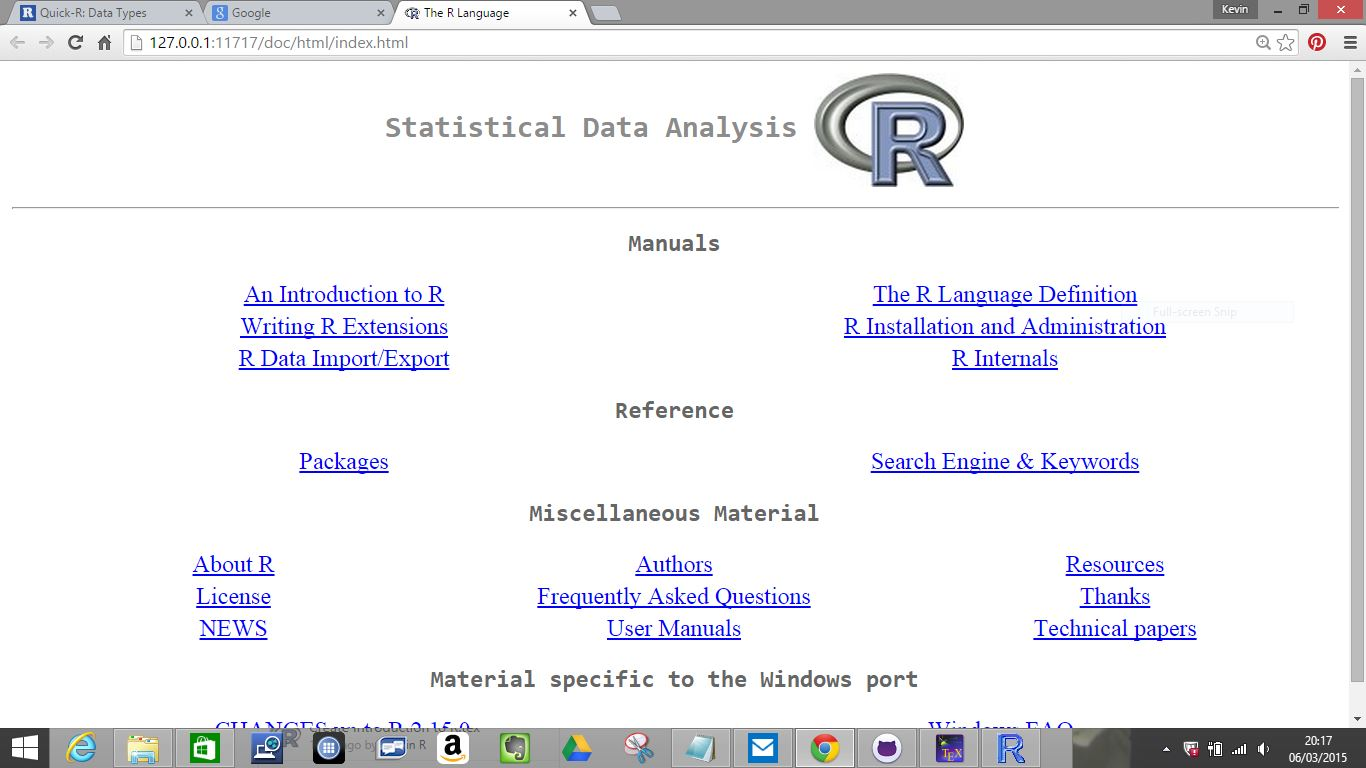
\includegraphics[width=1.2\linewidth]{images/helpstart}

\end{figure}

%===


{1.8 Basic Maths Operations}
\vspace{-0.5cm}
The most commonly used mathematical operators are all supported by ``R}. \\  Here are a few
examples:
\begin{tabular}{|c|c|} \hline
$5 + 3 \ast 5$ &  Note the order of operations.\\\hline
log (10) & Natural logarithm with base e=2.718282 \\\hline
log(8,2) & Log to the base 2 \\\hline
$4^2$ & 4 raised to the second power \\\hline
7/2 & Division \\\hline
factorial(4) & Factorial of Four \\\hline
sqrt (25) & Square root \\\hline
abs (3-7) & Absolute value of 3-7 \\\hline
pi & The mysterious number \\\hline
exp(2) & exponential function \\\hline

\end{tabular} 


%===


``R} can be used for many mathematical operations, including


* Set Theory
* Trigonometry
* Complex Numbers
* Binomial Coefficients

Set Theory is always useful to know (Monty Hall Problem). We will not go into any of the others in great detail today.


%===

{1.9 Basic ``R} Editor}

* ``R} has an inbuilt script editor. We will use it for this class, but there are plenty of top quality
Integrated Development Environments out there. (Read up about \textbf{RStudio} for example).
* For a while, we will use the in-built script editor. Although it is advisable to start using \textbf{Rstudio} or something similar in the not-too-distant future.




%===

% % SLIDE 1 - COVER SLIDE
\begin{figure}
\centering
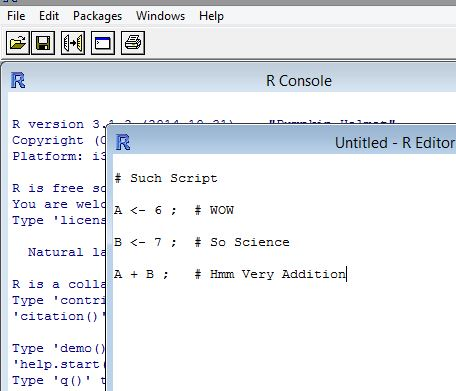
\includegraphics[width=1.2\linewidth]{images/Rscript}         
\end{figure}
   
%===

{1.9 Basic ``R} Editor}

* To start a new script, or open an existing script simply go to File and click the appropriate
options. A new dialogue box will appear. 

* You can write and edit code using this editor.
* To pass the code for compiling , press the run line or selection option (The third icon
on the menu).


%===



* Another way to read code is to use the ``edit()`` function, which operates directly from the
command line. 
* To see how the code defining an object X was written (or more importantly,
could have been written) simply type ``edit(X)}. 
* This command has some useful applications
that we will see later on (the ``scan()`` command).



%===



